\documentclass[12 pt]{article}

% Basic
\usepackage[utf8]{inputenc}
% \usepackage[spanish,mexico]{babel}

% Don't indent paragraphs, leave some space between them
\usepackage{parskip}
\usepackage{enumitem}
\usepackage{graphicx}
\usepackage{subfig}

% Math stuff
\usepackage{amsmath, amsfonts, mathtools, amsthm, amssymb}
\usepackage{breqn}
\usepackage{cancel}
\usepackage{etoolbox}
\usepackage{float}


% For neural networks
\usepackage{tikz}
\usetikzlibrary{matrix,chains,positioning,decorations.pathreplacing,arrows}

% Headers
\usepackage{fancyhdr}
\usepackage{lastpage}
\pagestyle{fancy}
\setlength{\headheight}{40pt}

% Commands
\newcommand\N{\ensuremath{\mathbb{N}}}
\newcommand\R{\ensuremath{\mathbb{R}}}
\newcommand\Z{\ensuremath{\mathbb{Z}}}
\newcommand\Q{\ensuremath{\mathbb{Q}}}
\newcommand\C{\ensuremath{\mathbb{C}}}

%Images
\usepackage{import}
\usepackage{xifthen}
\usepackage{pdfpages}
\usepackage{transparent}

\newcommand{\incfig}[1]{%
    \def\svgwidth{\columnwidth}
    \scalebox{.75}{\import{./figures/}{#1.pdf_tex}}
}

\newtheorem{teo}{Teorema}
\newtheorem{lema}{Lemma}

\newenvironment{solution}
  {\renewcommand\qedsymbol{$\blacksquare$}
  \begin{proof}[Proof]}
  {\end{proof}}
\renewcommand\qedsymbol{$\blacksquare$}


\begin{document}

\lhead{Hyperparameter tuning, Regularization \\ and Optimization}
\rhead{ Deep Learning specialization}
\cfoot{\thepage \ of \pageref{LastPage}}

Since deep learning is a highly empirical and iterative process, it's really helpfull 
to train models quickly. Having fast optimization algorithms is important and can
really speed up the efficiency of the process.

\section*{Mini-batch gradient descent}

Instead of processing the entire dataset all at the same time in mini-batch gradient we
partition the dataset in $N$ smaller subsets, then each subset $(X^{[t]}, Y^{[t]})$ of 
the dataset are processed.

When every subset of the dataset is processed we say that we did "1 epoch" or one single
pass through the training set. Usually several epochs are made.

Mini-batch gradient descent is considerably faster than normal gradient descent. A 
comparison between the cost functions of batch and mini-batch gradient descent is given 
in the following image:

\begin{figure}[H]
    \begin{center}
            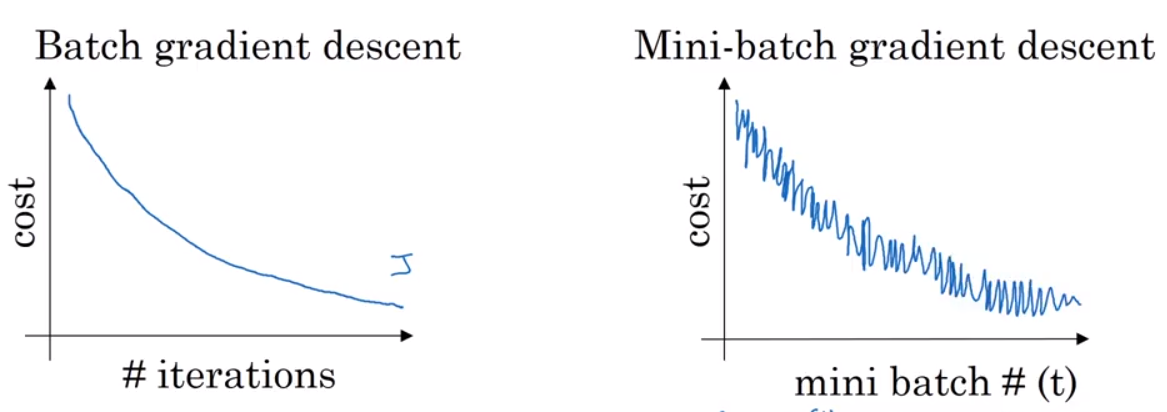
\includegraphics[width=0.9\textwidth]{img/minibatch.png}
            \caption{Batch vs Mini-batch gradient descent cost function}
        \end{center}
\end{figure}

\textbf{Differente mini-batch sizes}
\begin{itemize}
    \item mini-batch size $m$ : Batch gradient descent.
    \item mini-batch size $1$ : Stochastic gradient descent.
\end{itemize}

In practice the best mini-batch size should be between $1$ and $m$; if you take mini-batch
size $m$ then it takes too long to train the neural network, in the other case taking
size = $1$ is really noisy and losses almost all the speed of doing vectorization.

\begin{figure}[H]
    \begin{center}
            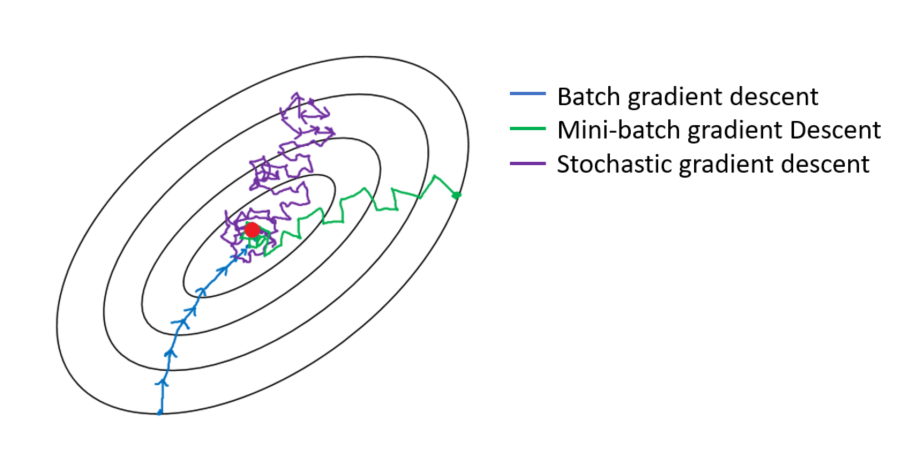
\includegraphics[width=0.9\textwidth]{img/descent.png}
            \caption{Comparison between mini-batch sizes}
        \end{center}
\end{figure}

\textbf{Which mini-batch size to choose?}
\begin{itemize}
    \item If the training set is small use batch gradient descent
    \item In any other case, typical mini-batch sizes are: $64,128,256,512,1024$. They're 
    all powers of two because of the way computer memory is layed out and accessed, 
    sometimes the code runs faster if the mini-batch size is a power of 2.
\end{itemize}

\section*{Exponentially weighted averages}

Exponentially weighted averages is a technique for smoothing time series data using the
exponential window function. Let's say we have a sequence $\{x_t\}_{t=0}^n$, the output
of the exponentially weighted averages is $\{v_t\}_{t=0}^n$ where:
\begin{align*}
    v_0 &= x_0 \\
    v_i &= \beta v_{i-1} + (1-\beta) x_i  && \forall i>0
\end{align*}

Where $\beta$ is the smoothing factor, $0 < \beta < 1$ 
\begin{figure}[H]
    \begin{center}
            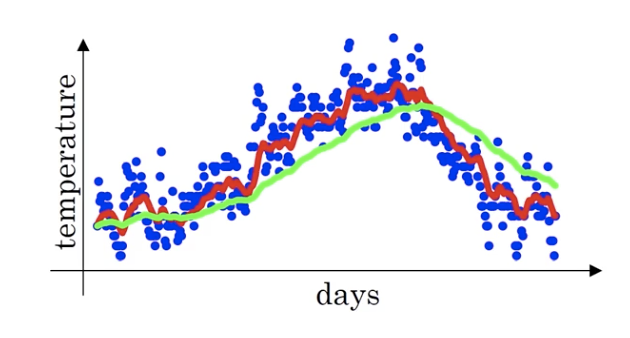
\includegraphics[width=0.9\textwidth]{img/es.png}
            \caption{Comparison between different smoothing factors}
        \end{center}
\end{figure}

The green line is for a greater $\beta$ and the red line for a smaller $\beta$, in general
the bigger the value of the smoothing factor the longer it takes for the exponentially 
weighted average to adapt.

Notice that in general $v_i$ can be expressed as follows:

\begin{align*}
    v_i &= \beta v_{i-1} + (1-\beta) x_i \\
        &= (1-\beta) x_i + \beta(1-\beta) x_{i-1} + \beta^2 v_{i-2} \\
        & \quad \vdots \\
        &= (1-\beta) x_i + \beta(1-\beta) x_{i-1} + \beta^2(1-\beta)x_{i-2} + \dots + \beta^i(1-\beta)x_0\\
        &= \sum_{k=0}^i \beta^{i-k} (1-\beta) x_i
\end{align*}

That means that we have an exponentially decaying function.

\textbf{Bias correction in exponentially weighted averages}

While computing the value og the exponentially weighted averages for small values of $t$
there's a bias because we have few observations and for big value of $\beta$ the 
algorithm may take a while to react to the inicialization. A way to correct this is by
changing $v_t$ with the following expression:
\begin{align*}
    v_t^* := \frac{v_t}{1-\beta^t}
\end{align*}
Notice that as $t$ grows $v_t^*$ approaches $v_t$.

\section*{Gradient descent with momentum}

Usually this algorithm is faster than the standard gradient descent procedure. The idea
is to compute an exponentially weighted average of the gradients and then use that
to update the weights instead. Formally, Compute $dW, db$ normally with the current 
mini-batch, then:
\begin{align*}
    V_{dW} &= \beta V_{dW} + (1 - \beta)dW \\
    V_{db} &= \beta V_{db} + (1 - \beta)db \\
    W &= W - \alpha V_{dW} \\
    b &= b - \alpha V_{db}
\end{align*}
Supose that when using the standard gradient descent you get a lot of oscilations 
when converging to the optimal value, using momentum can fix this because you are taking
into consideration the former results of the gradient therefore the oscilation starts
to decrease and the covergence is faster.

\textbf{Intuition:} in the convex combination of $V_{dW}$ and $dW$ the derivative term
represents the acceleration in the current point but the momentum term let's you take
into consideration the path traveled before.

Notice that now you have another Hyperparameter, $\beta$. Usually $\beta = .9$ works 
pretty well.

\section*{RMSprop}

RMSprop, which stands for root mean square prop is another algorithm that can speed up
gradient descent, on iteration $t$ we would compute $dW, db$ normally with the current 
mini-batch and then do the following calculation:
\begin{align*}
    S_{dW} &= \beta S_{dW} + (1 - \beta)dW^2 \\
    S_{db} &= \beta S_{db} + (1 - \beta)db^2 \\
    W &= W - \alpha \frac{dW}{\sqrt{S_{dW}}} \\
    b &= b - \alpha \frac{db}{\sqrt{S_{db}}}
\end{align*}

Observation: Using RMSprop makes it posible to use a higher learning rate and perform
faster learning without diverging

\section*{Adam}
Adam algorithm has been chown to work wll across a wide range of deep learning architectures,
the basic idea is to combine momentum and RMSprop. On iteration $t$ we would compute $dW, db$ normally with the current 
mini-batch and then do the following:
\begin{align*}
    & \text{Compute momentum and RMSprop:} \\
    & V_{dW} = \beta_1 V_{dW} + (1 - \beta_1)dW  && V_{db} = \beta_1 V_{db} + (1 - \beta_1)db \\
    & S_{dW} = \beta_2 S_{dW} + (1 - \beta_2)dW^2 && S_{db} = \beta_2 S_{db} + (1 - \beta_2)db^2 \\ \\
    & \text{Perform bias correction:} \\
    & V_{dW}^{\text{corr}} = \frac{V_{dW}}{1-\beta_1^t} && V_{db}^{\text{corr}} = \frac{V_{db}}{1-\beta_1^t} \\
    & S_{dW}^{\text{corr}} = \frac{S_{dW}}{1-\beta_2^t} && S_{db}^{\text{corr}} = \frac{S_{db}}{1-\beta_2^t} \\ \\
    & \text{Perform the update:} \\
    & W = W - \alpha \frac{V_{dW}^{\text{corr}}}{\sqrt{S_{dW}^{\text{corr}}}} \\
    & b = b - \alpha \frac{V_{db}^{\text{corr}}}{\sqrt{S_{db}^{\text{corr}}}} \\
\end{align*}

Hyperparameters choice:
\begin{itemize}
    \item $\alpha : \text{ needs to be tuned}$
    \item $\beta_1 : .9$ 
    \item $\beta_2 : .999$
\end{itemize}
The betas can be tuned but usually those default values are used.

\section*{Learning rate decay}
One of the things that might help speed up the learning algorithm, is to slowly reduce 
the learning rate over time. The idea is that during the initial phases while the learning rate 
alpha is still large, the algorithm shows a relatively fast learning. But then as alpha 
gets smaller, the steps it takes will be slower and smaller. And so it ends up oscillating 
in a tighter region around the minimum. If you never reduce the learning rate you might
oscilate a lot around the minimum without converging at all.

The most used formula to compute the learning rate is the following:
\begin{align*}
    \alpha = \frac{1}{1 + \text{decay\_rate}*\text{epoch}}
\end{align*}

Other learning rate decay methods:
\begin{align*}
    \alpha = .95^{\text{epoch}}\alpha_0 && \text{exponentially decay} \\
    \alpha = \frac{k}{\sqrt{\text{epoch}}}\alpha_0 && \text{constant decay} 
\end{align*}

\end{document}